\documentclass[11pt]{article}
\usepackage[a4paper,margin=1in]{geometry}
\usepackage[T1]{fontenc}
\usepackage[utf8]{inputenc}
\usepackage{lmodern}
\usepackage{amsmath,amssymb,amsthm,mathtools,bm}
\usepackage{microtype}
\usepackage{xcolor}
\usepackage{booktabs}
\usepackage{tikz}
\usetikzlibrary{arrows.meta,positioning,calc,decorations.markings,shapes.geometric,fit}
\usepackage[hidelinks]{hyperref}

\newtheorem{theorem}{Theorem}
\newtheorem{proposition}{Proposition}
\newtheorem{lemma}{Lemma}
\newtheorem{remark}{Remark}
\newtheorem{definition}{Definition}

\newcommand{\E}{\mathbb E}
\newcommand{\Var}{\operatorname{Var}}
\newcommand{\Cov}{\operatorname{Cov}}
\newcommand{\cum}{\operatorname{cum}}
\newcommand{\Tr}{\operatorname{Tr}}
\newcommand{\op}{\operatorname{op}}
\newcommand{\dd}{\mathrm d}
\newcommand{\cK}{\mathcal K}
\newcommand{\cT}{\mathcal T}
\newcommand{\cV}{\mathcal V}
\newcommand{\cA}{\mathcal A}
\newcommand{\cC}{\mathcal C}
\newcommand{\cP}{\mathcal P}
\newcommand{\cR}{\mathcal R}
\newcommand{\cG}{\mathcal G}
\newcommand{\btheta}{\boldsymbol\theta}
\newcommand{\eps}{\varepsilon}
\newcommand{\one}{\mathbf 1}
\newcommand{\diag}{\operatorname{diag}}

\tikzset{
  ext/.style={circle,fill=black,inner sep=1.7pt},
  extblue/.style={circle,fill=blue!70!black,inner sep=1.7pt},
  extred/.style={circle,fill=red!70!black,inner sep=1.7pt},
  det/.style={circle,draw=blue!70!black,fill=blue!8,minimum size=7mm,inner sep=1pt},
  rankv/.style={rectangle,draw=orange!80!black,fill=orange!15,rounded corners=2pt,minimum width=7mm,minimum height=5mm,inner sep=1pt},
  haarv/.style={diamond,draw=purple!80!black,fill=purple!12,aspect=1.4,minimum width=8mm,minimum height=6mm,inner sep=1pt},
  sourcev/.style={rectangle,draw=black,fill=gray!10,minimum width=7mm,minimum height=5mm,inner sep=1pt},
  proj/.style={rectangle,draw=red!70!black,fill=red!8,minimum width=6mm,minimum height=5mm,inner sep=1pt},
  solid/.style={line width=.85pt,black},
  ntk/.style={line width=.9pt,dashed,blue!70!black},
  dntk/.style={line width=.9pt,densely dotted,purple!80!black},
  detedge/.style={line width=.9pt,green!50!black,-{Stealth[length=2mm]}},
  rankedge/.style={line width=.85pt,orange!80!black},
  hairedge/.style={line width=.85pt,purple!80!black},
  kill/.style={line width=1pt,red!70!black},
  lab/.style={font=\scriptsize},
  every picture/.style={baseline={(current bounding box.center)}}
}

\title{Low-Rank Diagrammatic Rules for Finite-Rank NTK Corrections\\
\large A graphical calculus replacing full-width neural-index Feynman diagrams by rank cumulant vertices}
\author{Technical note for the low-rank NTK manuscript}
\date{\today}

\begin{document}
\maketitle

\begin{abstract}
The finite-width Feynman diagram formalism for MLP NTKs uses external preactivation, NTK, dNTK and ddNTK lines, cubic interaction vertices, Gaussian propagators, and quartic tensors $V,D,F,A,B$ together with descendants $P,Q,R,S,T,U$.  This note writes the analogous graphical calculus for the low-rank setting considered in our manuscript.  The central simplification is that stochasticity from a rank-$r$ bottleneck is represented by cumulants of an empirical rank state
\[
M_A^{(\ell)}=\frac1r\sum_{a=1}^r\phi_A^{(\ell)}(Z_a),
\]
so that a connected vertex of valence $s$ carries the exact weight $r^{1-s}$.  In the isometric model
\[
W^{(\ell)}=\frac{\sigma_w}{\sqrt{n_{\ell-1}}}\sqrt{\frac{n_\ell}{r_\ell}}\,U^{(\ell)}B^{(\ell)},\qquad U^{(\ell)\top}U^{(\ell)}=I_{r_\ell},
\]
rank-defect vertices are cumulants of the normalized Haar projector $G=(n/r)UU^\top$, whose second cumulant is exactly proportional to
\[
\gamma_{n,r}=\frac{n(n-r)}{r(n-1)(n+2)}\sim \frac1r-\frac1n.
\]
When $r=n$, $G=I$ and all rank-defect vertices vanish; the network is a pathwise orthogonal reparametrization of the full MLP.  In the RF-LR bottleneck regime, the same diagrams acquire a transport factor $(1/r)\dot\Sigma$, producing geometric memory suppression of old NTK lines.  The note gives explicit diagram rules, examples, and the centered RF-LR memory lemma in diagrammatic form.
\end{abstract}

\tableofcontents

\section{Why a new diagrammatic calculus is needed}

The finite-width Feynman paper gives a full set of graphical rules for NTK statistics: solid external lines for preactivations, dotted external lines for NTK fluctuations, higher dotted structures for dNTK and ddNTK, cubic interaction vertices, Gaussian propagators, and quartic vertices for the tensors $V,D,F,A,B$; it also extends the rules to $P,Q,R,S,T,U$ and all higher orders.  Our low-rank setting has the same external objects, but the internal randomness has a different origin.  Instead of summing unconstrained neural indices and then organizing Kronecker pairings, the bottleneck exposes a finite empirical rank average.  Therefore the basic random vertex is not a neural-index vertex; it is a cumulant of the rank state.

The purpose of this note is to state the graphical rules explicitly.  The slogan is
\[
\boxed{\text{full-width diagrams: neural-index contractions and Gaussian propagators}}
\]
whereas
\[
\boxed{\text{low-rank diagrams: empirical-rank cumulant vertices and deterministic layer derivatives}.}
\]
The external grammar is deliberately kept close to the Feynman paper, but the internal stochastic vertices are replaced by rank cumulants.

\section{Two models and one notation}

We distinguish two architectures.  The first is the \emph{isometric MLP-compatible low-rank model}.  A hidden layer has
\begin{equation}
W^{(\ell)}=\frac{\sigma_w}{\sqrt{n_{\ell-1}}}\sqrt{\frac{n_\ell}{r_\ell}}\,U^{(\ell)}B^{(\ell)},
\qquad U^{(\ell)\top}U^{(\ell)}=I_{r_\ell},
\label{eq:isometric}
\end{equation}
with $U^{(\ell)}$ frozen and $B^{(\ell)}$ trained.  If $r_\ell=n_\ell$, then $U^{(\ell)}$ is square orthogonal and $B\mapsto UB$ is an isometry.  Hence the empirical NTK is exactly the full-rank MLP NTK, path by path.

The second is the \emph{RF-LR bottleneck model}.  Its limiting NTK recursion has explicit bottleneck prefactors,
\begin{equation}
\Theta^{(\ell)}(x,x')=1+\frac1r\Theta^{(\ell-1)}(x,x')\dot\Sigma^{(\ell)}(x,x')+\frac1r\Sigma^{(\ell)}(x,x').
\label{eq:rflr-rec}
\end{equation}
For ReLU at the edge of chaos, $\dot\Sigma^{(\ell)}\to 1/2$ along aligned off-diagonal pairs, so old NTK lines are transported with approximately $(2r)^{-1}$ per further layer.  This is the source of geometric memory suppression.

Throughout, we write
\[
P=I-\frac{\one\one^\top}{m}
\]
for centering on a dataset of size $m$.

\section{Visual dictionary}

\subsection{External observable lines}

The external lines are the same objects as in the full-width Feynman formalism.  A solid line is a preactivation or NNGP-type observable.  A dashed blue line is an NTK fluctuation.  A dotted purple line denotes a derivative-NTK descendant; double or triple descendants are represented by multiple dotted legs.

\begin{center}
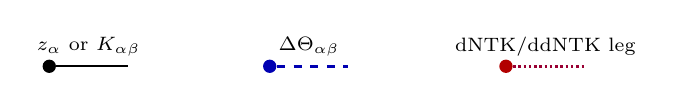
\begin{tikzpicture}[scale=1]
  \node[ext] (z0) at (0,0) {};
  \draw[solid] (z0) -- (1,0);
  \node[lab] at (.5,.25) {$z_\alpha$ or $K_{\alpha\beta}$};

  \node[extblue] (t0) at (2.8,0) {};
  \draw[ntk] (t0) -- (3.8,0);
  \node[lab] at (3.3,.25) {$\Delta\Theta_{\alpha\beta}$};

  \node[extred] (d0) at (5.8,0) {};
  \draw[dntk] (d0) -- (6.8,0);
  \node[lab] at (6.3,.25) {dNTK/ddNTK leg};
\end{tikzpicture}
\end{center}

\subsection{Deterministic layer-map vertices}

Let $\mathcal X_\ell$ collect the deterministic objects propagated through a layer: $K_\ell$, $\Theta_\ell$, and if needed dNTK/ddNTK descendants.  A layer is a deterministic map
\[
\mathcal X_{\ell+1}=\Phi_\ell(\mathcal X_\ell;M^{(\ell)},G^{(\ell)}).
\]
Derivatives of $\Phi_\ell$ are deterministic vertices.  They do not carry powers of $r$ or $n$; all stochastic scaling is carried by cumulant vertices.

\begin{center}
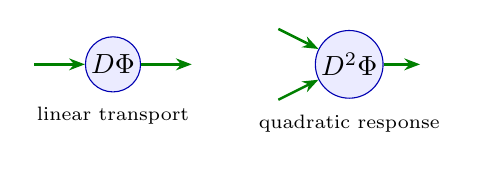
\begin{tikzpicture}[scale=1]
  \node[det] (D) at (0,0) {$D\Phi$};
  \draw[detedge] (-1,0)--(D);
  \draw[detedge] (D)--(1,0);
  \node[lab] at (0,-.65) {linear transport};

  \node[det] (D2) at (3,0) {$D^2\Phi$};
  \draw[detedge] (2.1,.45)--(D2);
  \draw[detedge] (2.1,-.45)--(D2);
  \draw[detedge] (D2)--(3.9,0);
  \node[lab] at (3,-.75) {quadratic response};
\end{tikzpicture}
\end{center}

\subsection{Rank cumulant vertices}

Let
\begin{equation}
M_A^{(\ell)}=\frac1r\sum_{a=1}^r\phi_A^{(\ell)}(Z_a),
\label{eq:rank-state}
\end{equation}
where $A$ labels an atom such as $\sigma\sigma$, $\sigma\sigma'$, $\sigma'\sigma'$, or a derivative analogue.  The rank atoms $Z_a$ are conditionally iid.  Hence
\begin{equation}
\cum(M_{A_1},\ldots,M_{A_s})=r^{1-s}\kappa_{A_1\cdots A_s},
\qquad
\kappa_{A_1\cdots A_s}:=\cum(\phi_{A_1}(Z),\ldots,\phi_{A_s}(Z)).
\label{eq:rank-cumulant}
\end{equation}
The diagram is a square rank vertex of valence $s$:

\begin{center}
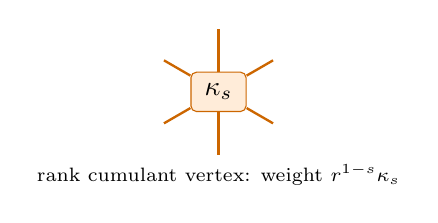
\begin{tikzpicture}[scale=1]
  \node[rankv] (R) at (0,0) {$\kappa_s$};
  \foreach \ang in {30,90,150,210,270,330}{
    \draw[rankedge] (R) -- ++(\ang:0.8);
  }
  \node[lab] at (0,-1.05) {rank cumulant vertex: weight $r^{1-s}\kappa_s$};
\end{tikzpicture}
\end{center}

This vertex is the central simplification of the low-rank calculus.

\subsection{Haar-projector vertices for the isometric model}

In the isometric model, rank-defect corrections are encoded by
\[
G=\frac nr UU^\top,
\qquad U^\top U=I_r.
\]
The second cumulant is exactly
\begin{equation}
\Cov(G_{ij},G_{kl})
=\gamma_{n,r}\left(\delta_{ik}\delta_{jl}+\delta_{il}\delta_{jk}-\frac2n\delta_{ij}\delta_{kl}\right),
\qquad
\gamma_{n,r}=\frac{n(n-r)}{r(n-1)(n+2)}.
\label{eq:haar-cov}
\end{equation}
Higher cumulants are given by orthogonal Weingarten contractions.  Graphically, a Haar vertex is a purple diamond:

\begin{center}
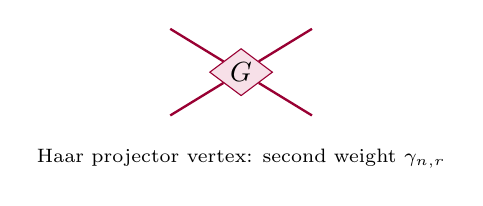
\begin{tikzpicture}[scale=1]
  \node[haarv] (H) at (0,0) {$G$};
  \draw[hairedge] (H)--(-.9,.55);
  \draw[hairedge] (H)--(-.9,-.55);
  \draw[hairedge] (H)--(.9,.55);
  \draw[hairedge] (H)--(.9,-.55);
  \node[lab] at (0,-1.1) {Haar projector vertex: second weight $\gamma_{n,r}$};
\end{tikzpicture}
\end{center}

When $r=n$, $G=I$ and every centered Haar cumulant vanishes.  Thus all rank-defect diagrams disappear.

\subsection{Centering projectors}

A red box $P$ projects out the constant dataset mode.  It is not a stochastic vertex; it is an external projection applied to the Gram operator.

\begin{center}
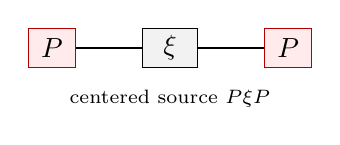
\begin{tikzpicture}[scale=1]
  \node[proj] (P1) at (0,0) {$P$};
  \node[sourcev] (S) at (1.5,0) {$\xi$};
  \node[proj] (P2) at (3,0) {$P$};
  \draw[solid] (P1)--(S)--(P2);
  \node[lab] at (1.5,-.65) {centered source $P\xi P$};
\end{tikzpicture}
\end{center}

This projector is essential in the RF-LR memory lemma: it kills or suppresses the radial constant mode responsible for diffusive $\sqrt L$ accumulation.

\section{The low-rank diagram rules}

\begin{definition}[Low-rank diagram]
A low-rank diagram is a finite graph built from:
\begin{enumerate}
\item external lines of type $z,K,\Theta,\mathrm d\Theta,\mathrm{dd}\Theta$;
\item deterministic Frechet vertices $D^q\Phi_\ell$;
\item rank cumulant vertices $\kappa_s$ with weight $r^{1-s}$;
\item optional Haar projector cumulant vertices with weights given by cumulants of $G=(n/r)UU^\top$;
\item transport edges $D\Phi_\ell$ along depth;
\item optional centering projectors $P$ on dataset Gram legs.
\end{enumerate}
A diagram is connected if all external lines are connected to the same stochastic cumulant component after contracting deterministic vertices.
\end{definition}

\begin{theorem}[Low-rank Feynman rules]
Let $F$ be a smooth observable of a finite number of layer states $M^{(\ell)}$ and Haar projectors $G^{(\ell)}$.  Its expansion in powers of $1/r$ and $\gamma_{n,r}$ is obtained by summing all low-rank diagrams with the prescribed external legs.  The algebraic value of a diagram is computed as follows.
\begin{enumerate}
\item Each rank vertex of valence $s$ contributes $r^{1-s}\kappa_s$.
\item Each Haar vertex contributes the corresponding cumulant of $G$; at valence two this is \eqref{eq:haar-cov}.
\item Each deterministic vertex contributes the corresponding derivative $D^q\Phi_\ell$ evaluated on the deterministic trajectory.
\item Each transport edge from layer $k$ to $L$ contributes the product of first derivatives along the path.  In RF-LR, an NTK transport edge contains the factor $(1/r)\dot\Sigma$ at each bottleneck layer.
\item For a cumulant, only connected diagrams are retained.  For a mean correction, vacuum subdiagrams are allowed but must be connected to the output by deterministic derivatives.
\end{enumerate}
\end{theorem}

\begin{proof}
The proof is the multivariate cumulant expansion for empirical averages.  For the rank state \eqref{eq:rank-state}, equation \eqref{eq:rank-cumulant} gives the exact cumulant scaling.  Applying Taylor's formula to $F(M)$ gives
\begin{equation}
\E F(M)=\left.\exp\left(\sum_{s\ge2}\frac{r^{1-s}}{s!}\kappa_{A_1\cdots A_s}\partial_{A_1}\cdots\partial_{A_s}\right)F(m)\right|_{m=\E M},
\label{eq:edgeworth}
\end{equation}
with higher-order remainders controlled by the corresponding smoothness norms.  Expanding the exponential gives exactly the diagram sum.  The Haar part is identical, replacing $r^{1-s}\kappa_s$ by orthogonal-projector cumulants.  Connected cumulants follow by the usual moment-cumulant cancellation: disconnected diagrams factor and are subtracted.
\end{proof}

\section{Basic diagrams}

\subsection{Mean correction}

For an observable $O=F(M)$, the first mean correction is the second derivative contracted against a rank two-point vertex:
\begin{equation}
\E O=F(m)+\frac1{2r}\kappa_{AB}\partial_A\partial_BF(m)+O(r^{-2}).
\end{equation}

\begin{center}
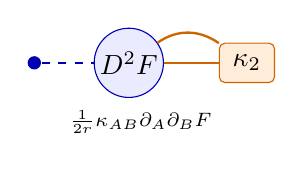
\begin{tikzpicture}[scale=1]
  \node[extblue] (out) at (0,0) {};
  \node[det] (D2) at (1.2,0) {$D^2F$};
  \node[rankv] (R) at (2.7,0) {$\kappa_2$};
  \draw[ntk] (out)--(D2);
  \draw[rankedge] (D2)--(R);
  \draw[rankedge] (D2) to[out=35,in=145] (R);
  \node[lab] at (1.35,-.75) {$\frac1{2r}\kappa_{AB}\partial_A\partial_BF$};
\end{tikzpicture}
\end{center}

In the isometric model one adds the analogous Haar two-point vertex, weighted by $\gamma_{n,r}$.

\subsection{NNGP covariance: the $V$ block}

The low-rank analogue of a four-preactivation connected cumulant is a covariance of rank-state insertions, transported by deterministic derivatives.

\begin{equation}
V_{\ell+1}=J^K_\ell V_\ell (J^K_\ell)^\top+\Xi^{KK}_\ell,
\qquad
\Xi^{KK}_\ell\equiv r^{-1}\kappa_2(S^K,S^K)+\gamma_{n,r}\,\mathfrak h^{KK}_\ell.
\label{eq:V-rec}
\end{equation}

\begin{center}
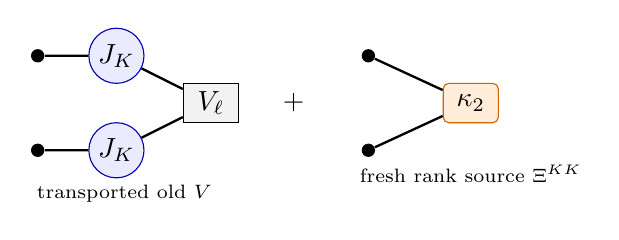
\begin{tikzpicture}[scale=1]
  % propagated old V
  \node[ext] (a) at (0,0.6) {};
  \node[ext] (b) at (0,-0.6) {};
  \node[det] (J1) at (1.0,0.6) {$J_K$};
  \node[det] (J2) at (1.0,-0.6) {$J_K$};
  \node[sourcev] (V) at (2.2,0) {$V_\ell$};
  \draw[solid] (a)--(J1)--(V);
  \draw[solid] (b)--(J2)--(V);
  \node[lab] at (1.1,-1.15) {transported old $V$};

  % plus
  \node at (3.25,0) {$+$};

  % fresh source
  \node[ext] (c) at (4.2,0.6) {};
  \node[ext] (d) at (4.2,-0.6) {};
  \node[rankv] (R) at (5.5,0) {$\kappa_2$};
  \draw[solid] (c)--(R);
  \draw[solid] (d)--(R);
  \node[lab] at (5.5,-.9) {fresh rank source $\Xi^{KK}$};
\end{tikzpicture}
\end{center}

\subsection{Mixed covariance: the $D,F$ block}

Let $C=(D,F)$ denote the mixed preactivation/NTK block.  Diagrammatically,
\begin{equation}
C_{\ell+1}=J^K_\ell C_\ell (J^\Theta_\ell)^\top + \text{source from }V_\ell + \Xi^{K\Theta}_\ell.
\label{eq:C-rec}
\end{equation}
The source from $V_\ell$ appears because the new NTK contains a fresh NNGP-like contribution.  The fresh low-rank source is a rank vertex with one solid and one dashed external leg.

\begin{center}
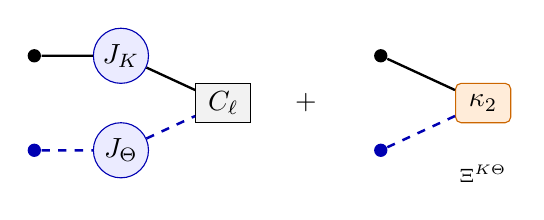
\begin{tikzpicture}[scale=1]
  \node[ext] (a) at (0,0.6) {};
  \node[extblue] (b) at (0,-0.6) {};
  \node[det] (Jk) at (1.1,0.6) {$J_K$};
  \node[det] (Jt) at (1.1,-0.6) {$J_\Theta$};
  \node[sourcev] (C) at (2.4,0) {$C_\ell$};
  \draw[solid] (a)--(Jk)--(C);
  \draw[ntk] (b)--(Jt)--(C);
  \node at (3.45,0) {$+$};
  \node[ext] (c) at (4.4,0.6) {};
  \node[extblue] (d) at (4.4,-0.6) {};
  \node[rankv] (R) at (5.7,0) {$\kappa_2$};
  \draw[solid] (c)--(R);
  \draw[ntk] (d)--(R);
  \node[lab] at (5.7,-.9) {$\Xi^{K\Theta}$};
\end{tikzpicture}
\end{center}

\subsection{NTK covariance: the $A,B$ block}

For $A=(A,B)$ one has
\begin{equation}
A_{\ell+1}=J^\Theta_\ell A_\ell (J^\Theta_\ell)^\top + \text{terms from }C_\ell,V_\ell +\Xi^{\Theta\Theta}_\ell.
\label{eq:A-rec}
\end{equation}
The leading fresh source is a rank cumulant with two NTK external legs.

\begin{center}
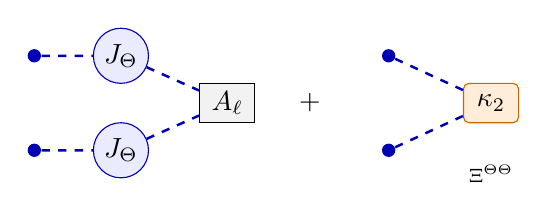
\begin{tikzpicture}[scale=1]
  \node[extblue] (a) at (0,0.6) {};
  \node[extblue] (b) at (0,-0.6) {};
  \node[det] (J1) at (1.1,0.6) {$J_\Theta$};
  \node[det] (J2) at (1.1,-0.6) {$J_\Theta$};
  \node[sourcev] (A) at (2.45,0) {$A_\ell$};
  \draw[ntk] (a)--(J1)--(A);
  \draw[ntk] (b)--(J2)--(A);
  \node at (3.5,0) {$+$};
  \node[extblue] (c) at (4.5,0.6) {};
  \node[extblue] (d) at (4.5,-0.6) {};
  \node[rankv] (R) at (5.8,0) {$\kappa_2$};
  \draw[ntk] (c)--(R);
  \draw[ntk] (d)--(R);
  \node[lab] at (5.8,-.9) {$\Xi^{\Theta\Theta}$};
\end{tikzpicture}
\end{center}

\section{The low-rank analogue of the five diagrams for $\Theta^{\{1\}}$}

In the full-width Feynman formalism, the first correction to the NTK mean has five order-$1/n$ diagrams: propagation of $\Theta^{\{1\}}$, insertion of $K^{\{1\}}$, and three quartic sources involving $V,D,F$.  In the low-rank calculus the external five-diagram pattern remains, but the internal quartic sources are themselves resolved into rank/Haar cumulant vertices.

\begin{equation}
\Theta^{\{1\}}_{\ell+1}
=\mathsf T_\Theta[\Theta^{\{1\}}_\ell]
+\mathsf T_K[K^{\{1\}}_\ell]
+\mathsf S_V[V_\ell]
+\mathsf S_D[D_\ell]
+\mathsf S_F[F_\ell].
\label{eq:theta-five}
\end{equation}

\begin{center}
\resizebox{\linewidth}{!}{%
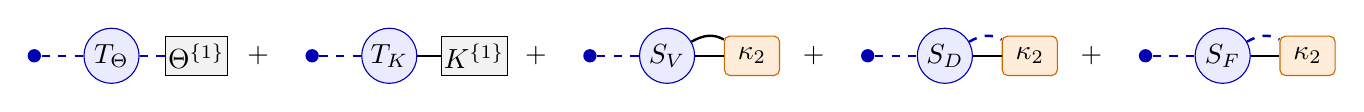
\begin{tikzpicture}[scale=.98]
  \node[extblue] (o1) at (0,0) {};
  \node[det] (t1) at (1,0) {$T_\Theta$};
  \node[sourcev] (th) at (2.1,0) {$\Theta^{\{1\}}$};
  \draw[ntk] (o1)--(t1)--(th);
  \node at (2.9,0) {$+$};

  \node[extblue] (o2) at (3.6,0) {};
  \node[det] (t2) at (4.6,0) {$T_K$};
  \node[sourcev] (kk) at (5.7,0) {$K^{\{1\}}$};
  \draw[ntk] (o2)--(t2);
  \draw[solid] (t2)--(kk);
  \node at (6.5,0) {$+$};

  \node[extblue] (o3) at (7.2,0) {};
  \node[det] (sv) at (8.2,0) {$S_V$};
  \node[rankv] (rv) at (9.3,0) {$\kappa_2$};
  \draw[ntk] (o3)--(sv);
  \draw[solid] (sv)--(rv);
  \draw[solid] (sv) to[out=30,in=150] (rv);

  \node at (10.1,0) {$+$};
  \node[extblue] (o4) at (10.8,0) {};
  \node[det] (sd) at (11.8,0) {$S_D$};
  \node[rankv] (rd) at (12.9,0) {$\kappa_2$};
  \draw[ntk] (o4)--(sd);
  \draw[solid] (sd)--(rd);
  \draw[ntk] (sd) to[out=30,in=150] (rd);

  \node at (13.7,0) {$+$};
  \node[extblue] (o5) at (14.4,0) {};
  \node[det] (sf) at (15.4,0) {$S_F$};
  \node[rankv] (rf) at (16.5,0) {$\kappa_2$};
  \draw[ntk] (o5)--(sf);
  \draw[solid] (sf)--(rf);
  \draw[ntk] (sf) to[out=30,in=150] (rf);
\end{tikzpicture}%
}
\end{center}

\noindent
The algebraic distinction from the full-width diagrams is that the source vertices $V,D,F$ can be expanded further into rank cumulants and Haar vertices.  Thus the low-rank calculus is not a different set of external tensors; it is a simpler internal expansion of their sources.

\section{Pairing extraction and tensor coefficients}

A rank-four neural tensor invariant under orthogonal changes decomposes as
\begin{equation}
C_{i_1i_2i_3i_4}
=c_1\delta_{i_1i_2}\delta_{i_3i_4}
+c_2\delta_{i_1i_3}\delta_{i_2i_4}
+c_3\delta_{i_1i_4}\delta_{i_2i_3}.
\label{eq:pairing}
\end{equation}
Let $B_1,B_2,B_3$ denote the three pairings.  Their normalized Gram matrix is
\begin{equation}
\overline G_N=
\begin{pmatrix}
1&1/N&1/N\\
1/N&1&1/N\\
1/N&1/N&1
\end{pmatrix},
\qquad
\overline G_N^{-1}=\frac{N}{N-1}I_3-\frac{N}{(N-1)(N+2)}\one\one^\top.
\label{eq:pairing-inv}
\end{equation}
Thus a measured triple of contractions $h=(\langle C,B_1\rangle,\langle C,B_2\rangle,\langle C,B_3\rangle)$ gives the actual coefficients by
\[
(c_1,c_2,c_3)^\top=\overline G_N^{-1}h.
\]
This is the diagrammatic extraction step missing from raw Gram-entry cumulant measurements.

\section{RF-LR memory suppression diagrams}

For RF-LR, an NTK line transported from layer $k$ to $L$ carries
\begin{equation}
B_{L:k}=\prod_{s=k+1}^L \frac1r\dot\Sigma^{(s)}.
\end{equation}
For ReLU at EOC, $\dot\Sigma^{(s)}\to 1/2$, hence
\begin{equation}
\|B_{L:k}\|\lesssim \left(\frac1{2r}\right)^{L-k}.
\end{equation}

\begin{center}
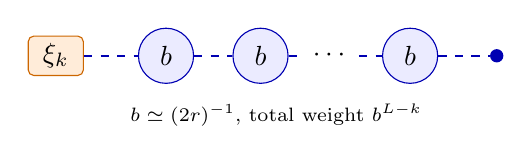
\begin{tikzpicture}[scale=1]
  \node[rankv] (S) at (0,0) {$\xi_k$};
  \node[det] (b1) at (1.4,0) {$b$};
  \node[det] (b2) at (2.6,0) {$b$};
  \node at (3.5,0) {$\cdots$};
  \node[det] (bL) at (4.5,0) {$b$};
  \node[extblue] (out) at (5.6,0) {};
  \draw[ntk] (S)--(b1)--(b2)--(3.15,0);
  \draw[ntk] (3.85,0)--(bL)--(out);
  \node[lab] at (2.8,-.75) {$b\simeq (2r)^{-1}$, total weight $b^{L-k}$};
\end{tikzpicture}
\end{center}

This geometric chain is the graphical origin of the improved centered RF-LR criterion.  The old contributions are not summed diffusively; they are exponentially localized near the output layer.

\section{Centered memory lemma in diagrams}

Let
\[
Z_L=P(\widehat K_L-K_L)P.
\]
The centered RF-LR fluctuation admits the linearized expansion
\begin{equation}
Z_L=\sum_{k=1}^L B_{L:k+1}Y_k+\sum_{k=1}^L B_{L:k+1}R_k,
\label{eq:centered-expansion}
\end{equation}
where $Y_k$ is a centered fresh rank source and $R_k$ is quadratic in previous fluctuations.  Diagrammatically:

\begin{center}
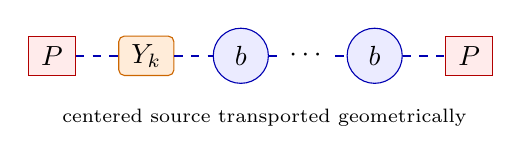
\begin{tikzpicture}[scale=1]
  \node[proj] (P1) at (-.7,0) {$P$};
  \node[rankv] (Y) at (.5,0) {$Y_k$};
  \node[det] (b1) at (1.7,0) {$b$};
  \node at (2.55,0) {$\cdots$};
  \node[det] (b2) at (3.4,0) {$b$};
  \node[proj] (P2) at (4.6,0) {$P$};
  \draw[ntk] (P1)--(Y)--(b1)--(2.2,0);
  \draw[ntk] (2.9,0)--(b2)--(P2);
  \node[lab] at (2,-.78) {centered source transported geometrically};
\end{tikzpicture}
\end{center}

\begin{lemma}[Centered RF-LR memory lemma]
Assume the centered source satisfies, conditionally on the past,
\begin{equation}
\left\|\E[Y_k^2\mid\mathcal F_{k-1}]\right\|_{\op}\le C\frac{m\eps_{\rm RF}}{r^2},
\qquad
\|Y_k\|_{\psi_1}\le C\frac{\sqrt{\eps_{\rm RF}}}{r},
\label{eq:Y-bound}
\end{equation}
and the transport satisfies $\|B_{L:k}\|\le q^{L-k}$ for some $q<1$.  Suppose also $\|R_k\|_{\op}\le C m\eps_{\rm RF}/r^2$ with high probability.  Then, up to logarithms, with probability at least $1-\delta$,
\begin{equation}
\|Z_L\|_{\op}\lesssim
\frac{\sqrt{m\eps_{\rm RF}\log(m/\delta)}}{r}
+
\frac{m\eps_{\rm RF}\log(m/\delta)}{r^2}.
\label{eq:centered-lemma}
\end{equation}
\end{lemma}

\begin{proof}
The martingale increments are $X_k=B_{L:k+1}Y_k$.  Their predictable variance is bounded by
\[
\left\|\sum_{k=1}^L\E[X_k^2\mid\mathcal F_{k-1}]\right\|_{\op}
\le
C\frac{m\eps_{\rm RF}}{r^2}\sum_{k=1}^Lq^{2(L-k)}
\le C'\frac{m\eps_{\rm RF}}{r^2}.
\]
Matrix Freedman/Bernstein gives the first term of \eqref{eq:centered-lemma}.  For the remainder,
\[
\left\|\sum_{k=1}^LB_{L:k+1}R_k\right\|_{\op}
\le C\frac{m\eps_{\rm RF}}{r^2}\sum_{k=1}^Lq^{L-k}
\le C'\frac{m\eps_{\rm RF}}{r^2}.
\]
This proves the claim.
\end{proof}

\begin{remark}[Why this does not apply to raw cumulants]
If the radial constant mode is not removed, one may have a recursion $R_{\ell+1}=R_\ell+\xi_{\ell+1}$, which gives $\Var(R_L)\sim L$.  This produces a diffusive factor $\sqrt L$ and returns the conservative condition.  The centered lemma is therefore a theorem about the centered/angularized RF-LR sector, not about raw NTK cumulants.
\end{remark}

\section{Spectral criterion from Weyl}

Let $K_L$ be the deterministic RF-LR proxy in the chosen normalization and $\widehat K_L$ its finite-rank/finite-width realization.  Weyl gives
\begin{equation}
\lambda_{\min}(P\widehat K_LP)\ge \lambda_{\min}(PK_LP)-\|P(\widehat K_L-K_L)P\|_{\op}.
\end{equation}
If
\begin{equation}
\lambda_{\min}(PK_LP)\ge \frac{c_{\rm data}}{rL}
\end{equation}
and the centered memory lemma holds, then it is sufficient that
\begin{equation}
\frac{\sqrt{m\eps_{\rm RF}}}{r}\lesssim \frac1{rL},
\end{equation}
that is
\begin{equation}
\eps_{\rm RF}\lesssim \frac1{mL^2}.
\end{equation}
When $\eps_{\rm RF}\simeq 1/r$, this becomes
\begin{equation}
\boxed{r\gtrsim mL^2.}
\end{equation}
The older $mL^3$ condition corresponds to replacing \eqref{eq:centered-lemma} by the diffusive raw bound $\|Z_L\|_{\op}\lesssim r^{-1}\sqrt{mL\eps_{\rm RF}}$.

\section{Comparison table}

\begin{center}
\begin{tabular}{@{}lll@{}}
\toprule
Regime & Fluctuation scale & Weyl criterion if $\mu\asymp (rL)^{-1}$ \\
\midrule
Raw/unprojected RF-LR & $r^{-1}\sqrt{mL\eps}$ & $\eps\lesssim (mL^3)^{-1}$ \\
Centered/angular RF-LR & $r^{-1}\sqrt{m\eps}$ & $\eps\lesssim (mL^2)^{-1}$ \\
If $\eps\simeq 1/r$ & - & $r\gtrsim mL^2$ \\
\bottomrule
\end{tabular}
\end{center}

\section{Flaw check}

\begin{enumerate}
\item The diagram rules do not claim that raw output NTK cumulants directly equal $V,D,F,A,B$.  One must extract pairings using \eqref{eq:pairing-inv}.
\item The centered RF-LR memory lemma assumes that $P$ removes the radial constant mode.  Without this projection, the $\sqrt L$ factor can reappear.
\item The $1/(rL)$ margin is normalization-dependent.  The invariant statement is $\Delta<\mu$, not a universal $1/(rL)$ law.
\item The isometric model and the RF-LR bottleneck model are distinct.  In the isometric model $r=n$ is full-rank MLP exactly.  In RF-LR, the kernel concentrates around its own proxy, not around the fully trained MLP NTK.
\item dNTK/ddNTK add derivative external legs but no new low-rank stochastic vertices; their diagrams are obtained by differentiating the deterministic vertices $D^q\Phi$.
\end{enumerate}

\section{Takeaway}

The low-rank graphical calculus is not a cosmetic rewrite of the full-width Feynman rules.  It changes the internal expansion parameter from neural-index contractions to empirical-rank cumulants.  The central new diagrams are:
\[
\begin{gathered}
\boxed{\text{rank cumulant vertices } r^{1-s}\kappa_s,}\qquad
\boxed{\text{Haar-projector vertices } \cum(G,\ldots,G),}\\[1mm]
\boxed{\text{RF-LR geometric transport } (r^{-1}\dot\Sigma)^{L-k}.}
\end{gathered}
\]
Together they explain the mixed expansion $1/n+\gamma_{n,r}$, exact matching at $r=n$, and the improvement from a conservative $mL^3$ rank criterion to the centered RF-LR criterion $mL^2$.

\end{document}
